\documentclass[notes,11pt, aspectratio=169]{beamer}

% { BEGIN_FOLD ---------- PREAMBLE -------------

\usepackage{pgfpages}
% These slides also contain speaker notes. You can print just the slides,
% just the notes, or both, depending on the setting below. Comment out the want
% you want.
\setbeameroption{hide notes} % Only slide
%\setbeameroption{show only notes} % Only notes
%\setbeameroption{show notes on second screen=right} % Both

\usepackage{helvet}
\usepackage[default]{lato}
\usepackage{array}

\usepackage[backend=biber,style=authoryear,
sorting=ynt,citestyle=authoryear]{biblatex}
\addbibresource{Paper/papercitations.bib}

\usepackage{tikz}
\usepackage{verbatim}
\setbeamertemplate{note page}{\pagecolor{yellow!5}\insertnote}
\usetikzlibrary{positioning}
\usetikzlibrary{snakes}
\usetikzlibrary{calc}
\usetikzlibrary{arrows}
\usetikzlibrary{decorations.markings}
\usetikzlibrary{shapes.misc}
\usetikzlibrary{matrix,shapes,arrows,fit,tikzmark}
\usepackage{amsmath}
\usepackage{mathpazo}
\usepackage{hyperref}
\usepackage{lipsum}
\usepackage{multimedia}
\usepackage{graphicx}
\usepackage{multirow}
\usepackage{booktabs}
\usepackage{dcolumn}
\usepackage{bbm}
\newcolumntype{d}[0]{D{.}{.}{5}}
\usepackage{subfigure}
\usepackage{import}
\usepackage{xcolor}

\usepackage{changepage}
\usepackage{appendixnumberbeamer}
\newcommand{\beginbackup}{
   \newcounter{framenumbervorappendix}
   \setcounter{framenumbervorappendix}{\value{framenumber}}
   \setbeamertemplate{footline}
   {
     \leavevmode%
     \hline
     box{%
       \begin{beamercolorbox}[wd=\paperwidth,ht=2.25ex,dp=1ex,right]{footlinecolor}%
%         \insertframenumber  \hspace*{2ex} 
       \end{beamercolorbox}}%
     \vskip0pt%
   }
 }
\newcommand{\backupend}{
   \addtocounter{framenumbervorappendix}{-\value{framenumber}}
   \addtocounter{framenumber}{\value{framenumbervorappendix}} 
}

\newcommand{\btVFill}{\vskip0pt plus 1filll}

\setbeamertemplate{blocks}[rounded]
\setbeamercolor{block title}{bg=purple, fg=white}
\setbeamercolor{block body}{bg=purple!10}

\usepackage{graphicx}
\usepackage[space]{grffile}
\usepackage{booktabs}

% These are my colors -- there are many like them, but these ones are mine.
\definecolor{sage}{RGB}{102,153,102}
\definecolor{yellow}{RGB}{255,173,1}
\definecolor{purple}{RGB}{153,102,153}

% colors for diagrams
\definecolor{diagramtan}{RGB}{225,190,106}
\definecolor{diagramteal}{RGB}{64, 176, 166}
\definecolor{diagrampurple}{RGB}{170, 131, 239}
\definecolor{diagramred}{RGB}{146, 79, 79}


\hypersetup{
  colorlinks=false,
  linkbordercolor = {white},
  linkcolor = {sage}
}


%% I use a beige off white for my background
\definecolor{MyBackground}{RGB}{255,253,218}

%% Uncomment this if you want to change the background color to something else
%\setbeamercolor{background canvas}{bg=MyBackground}

%% Change the bg color to adjust your transition slide background color!
\newenvironment{transitionframe}{
  \setbeamercolor{background canvas}{bg=white}
  \begin{frame}}{
    \end{frame}
}

\setbeamercolor{frametitle}{fg=sage}
\setbeamercolor{title}{fg=sage}
\setbeamertemplate{footline}[frame number]
\setbeamertemplate{navigation symbols}{} 
\setbeamertemplate{itemize items}{$\rightarrow$}
\setbeamertemplate{itemize subitem}{$\bullet$}
\setbeamercolor{itemize item}{fg=sage}
\setbeamercolor{itemize subitem}{fg=sage}
\setbeamercolor{enumerate item}{fg=sage}
\setbeamercolor{enumerate subitem}{fg=sage}
\setbeamercolor{button}{bg=sage,fg=white}



% If you like road maps, rather than having clutter at the top, have a roadmap show up at the end of each section 
% (and after your introduction)
% Uncomment this is if you want the roadmap!
\AtBeginSection[]
{
   \begin{frame}
       \frametitle{Roadmap of Talk}
       \tableofcontents[currentsection]
   \end{frame}
}
\setbeamercolor{section in toc}{fg=sage}
\setbeamercolor{subsection in toc}{fg=sage}
\setbeamersize{text margin left=1em,text margin right=1em} 

\newenvironment{wideitemize}{\itemize\addtolength{\itemsep}{10pt}}{\enditemize}

\usepackage{environ}
\NewEnviron{videoframe}[1]{
  \begin{frame}
    \vspace{-8pt}
    \begin{columns}[onlytextwidth, T] % align columns
      \begin{column}{.58\textwidth}
        \begin{minipage}[t][\textheight][t]
          {\dimexpr\textwidth}
          \vspace{8pt}
          \hspace{4pt} {\Large \sc \textcolor{blue}{#1}}
          \vspace{8pt}
          
          \BODY
        \end{minipage}
      \end{column}%
      \hfill%
      \begin{column}{.42\textwidth}
        \colorbox{green!20}{\begin{minipage}[t][1.2\textheight][t]
            {\dimexpr\textwidth}
            Face goes here
          \end{minipage}}
      \end{column}%
    \end{columns}
  \end{frame}
}

% } ---------- PREAMBLE -------------

\title[]{\textcolor{sage}{Does Hospital Leadership Matter? \\Evidence from Pay-for-Performance Incentives}}

\author[]{Hanna Glenn\\ \textit{Emory University}}
\date{\today}


\begin{document}

%%% { TIKZ STUFF
\tikzset{   
        every picture/.style={remember picture,baseline},
        every node/.style={anchor=base,align=center,outer sep=1.5pt},
        every path/.style={thick},
        }
\newcommand\marktopleft[1]{%
    \tikz[overlay,remember picture] 
        \node (marker-#1-a) at (-.3em,.3em) {};%
}
\newcommand\markbottomright[2]{%
    \tikz[overlay,remember picture] 
        \node (marker-#1-b) at (0em,0em) {};%
}
\tikzstyle{every picture}+=[remember picture] 
\tikzstyle{mybox} =[draw=black, very thick, rectangle, inner sep=10pt, inner ysep=20pt]
\tikzstyle{fancytitle} =[draw=black,fill=red, text=white]
%%%% } ------------ TIKZ STUFF ---------

% Title Slide
\begin{frame}
\maketitle
\end{frame}

\begin{frame}{Leader Characteristics Influence Firms}

    \vspace{5mm}

    \begin{wideitemize}
        \item Female executives correlated with female wages (\cite{flabbi2019female})
        \item Young male CEOs more aggressive in mergers (\cite{levi2010deal})
        \item Military CEOs less aggressive (\cite{benmelech2015military})
        \item General ability CEOs are at better performing firms than specialized ability (\cite{custodio2013generalists})
    \end{wideitemize}
    \btVFill \pause

    \begin{block}{Gap}
        \begin{itemize}
            \item What we know is typically in large, publicly traded firms
            \item Limited evidence in not-for-profit (NFP) settings with different incentives
        \end{itemize}
    \end{block}

\end{frame}

\begin{frame}{Not-for-Profit Behavior}

    \vspace{12mm}
    NFP objectives in general are unclear

    \vspace{8mm}
    \begin{wideitemize}
        \item Focus in research on understanding NFP hospitals: profit driven or not?
        \item NFP hospitals in the US: private but designated as NFP by taxes
        \begin{itemize}
            \item Make up majority of hospitals in the US
            \item Behavior has direct impact on patient population
        \end{itemize}
    \end{wideitemize}

    \btVFill \pause

    \begin{block}{This Paper}
        Examine whether executive team characteristics reveal NFP hospital behavior
        \begin{itemize}
            \item leverage exogenous shock to incentives: pay-for-performance
        \end{itemize}
    \end{block}

\end{frame}

\begin{frame}{Hospital Choice of Quality}
\vspace{5mm}
$$\max_{\theta}\hspace{2mm}\alpha\pi(\theta) + (1-\alpha) u(\theta)$$
\begin{itemize}
        \item $\theta$: quality
        \item $\pi(\theta)$: profit function 
        \item $u(\theta)$: patient/society benefit
        \item $\alpha\in\left[0,1\right]$: weight placed on profit function 
    \end{itemize}
    \btVFill

\end{frame}

\begin{frame}[noframenumbering]{Hospital Choice of Quality}
\vspace{5mm}
$$\max_{\theta}\hspace{2mm}\alpha\pi(\theta) + (1-\alpha) u(\theta)$$

    \vspace{3mm}

The US health care system is still largely fee-for-service
\begin{itemize}
    \item providers do not financially benefit from quality, only from quantity
    \item $\pi(\theta)$ is decreasing in $\theta$
\end{itemize}
    \begin{block}{}
        Quality is decreasing in $\alpha$ 
    \end{block}

\vspace{3mm}\pause

With pay-for-performance:
\begin{itemize}
    \item Hospitals are rewarded for high quality or penalized for low quality
    \item $\pi(\theta)$ is an increasing function with $\pi(\theta)\geq 0$
\end{itemize}
    \begin{block}{}
        Quality is increasing in $\alpha$ 
    \end{block}


    \btVFill
\end{frame}


\begin{frame}{Response to P4P}
\vspace{10mm}
    \begin{align*}
        \Delta\theta &= \theta_{P4P}-\theta\\
        \\
        \frac{d\Delta\theta}{d\alpha}&=\frac{d(\theta_{P4P}-\theta)}{d\alpha}\\
        &=\frac{d\theta_{P4P}}{d\alpha}-\frac{d\theta}{d\alpha}\\
        &\geq 0.
    \end{align*}
    \btVFill\pause

    \begin{block}{}
    Hospital response to P4P is increasing as more weight is placed on profit
    \end{block}
\end{frame}

\begin{frame}{This Paper}
\vspace{5mm}
\begin{wideitemize}
    \item Objectives reflected in $\alpha$: does leadership team help reveal these objectives?
    \item Debated characteristic of hospital leaders: clinical experience
    \begin{itemize}
        \item better understanding of patients
        \item lack of managerial experience (\cite{otero2022managers})
        \item could affect weight placed on profit vs. patients
    \end{itemize}
\end{wideitemize}

\btVFill\pause

\begin{block}{}
    I compare response to P4P between NFP hospitals with and without clinical executives
    \begin{itemize}
        \item I find that NFP hospitals without clinical executives respond more aggressively to P4P
    \end{itemize}\pause
\end{block}
\begin{block}{Mechanisms}
    \begin{itemize}
        \item Are clinical executives less profit driven?
        \item Are clinical executives a signal of underlying objectives or do they manage the hospital differently? 
    \end{itemize}
\end{block}
  
\end{frame}

\begin{frame}{Clinical Executives}
NFP executives are understudied partly because of difficulty identifying them

\vspace{4mm}

Scrape executive teams from public Tax Form 990s 

\vspace{4mm}

    \centering
    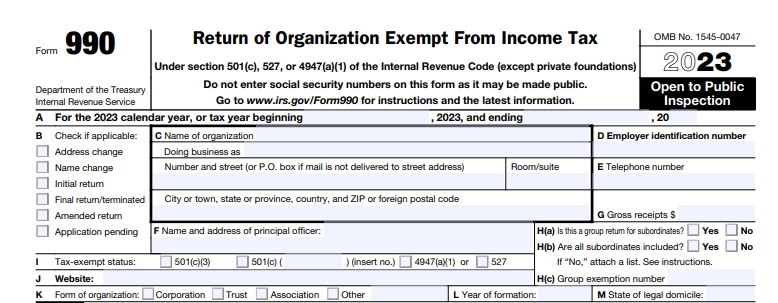
\includegraphics[width=.8\textwidth]{Graphics/990_snip_frontpage.PNG}
\end{frame}

\begin{frame}{Clinical Executives}
Section about executives and board members:
\begin{itemize}
                \item Use OCR text extraction algorithms to get names, positions, titles
                \item Limit to executives
            \end{itemize}

            \vspace{3mm}

\centering
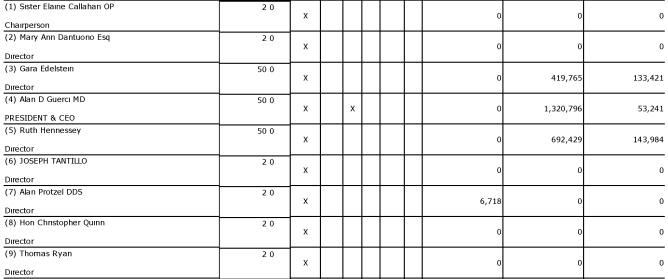
\includegraphics[width=.75\textwidth]{Graphics/990_snip_namesexample.PNG}
    
\end{frame}

\begin{frame}{Clinical Executives}\label{clinexecs}
    \vspace{10mm}
    \begin{wideitemize}
            \item Characterize NFP hospitals as having any executives trained as an MD
            \item Focus on stable teams
            \begin{itemize}
                \item don't change propensity to hire an MD over time
            \end{itemize}
            \item 521 NFP hospitals w/ stable teams 
            \begin{itemize}
                \item 10\% have MD exec
            \end{itemize}
    \end{wideitemize}
    \btVFill
    \hyperlink{990s}{\beamerbutton{getting data}} \hyperlink{execstats}{\beamerbutton{stats}}
\end{frame}

\begin{frame}{2012 Pay-for-Performance Policies}\label{policies}
    \vspace{7mm}

    Hospital Readmissions Reduction Program:
    \begin{itemize}
        \item Penalty for high readmissions for given conditions: heart attack, heart failure, pneumonia
        
    \end{itemize}

    \vspace{5mm}

    Hospital Value Based Purchasing Program:
    \begin{itemize}
        \item Rewarded based on quality compared to other hospitals and whether quality improves over time
    \end{itemize}

    \btVFill
    
    \hyperlink{policies}{\beamerbutton{policies}}
    
    \vspace{2mm}

    \begin{block}{}
        Exogenous shocks to hospitals: predetermined leadership teams are not correlated with the incentive change
    \end{block}
\end{frame}

\begin{frame}{Estimating the Effect of Clinical Executives on Quality after P4P}
\begin{equation*}
    y_{ht} = \beta \text{ treat}_{ht} + \gamma_{h} + \delta_t + \epsilon_{ht}
\end{equation*}

\vspace{3mm}

\begin{wideitemize}
    \item h: NFP hospitals in the US
    \begin{itemize}
        \item limit to general hospitals w/ stable executive teams
    \end{itemize}
    \item t: year $\in$ 2010-2014
    \item $y_{ht}$: Readmission and mortality rates
    \begin{itemize}
        \item I create a weighted average based on number of patients in each relevant condition
        \item data: government collection of hospital quality statistics (Hospital Compare)
    \end{itemize} 
    \item treat$_{ht}$: Has clinical executive x Post P4P
\end{wideitemize}
\btVFill
\begin{block}{}
    Ultimately employ a synthetic diff-in-diff
\end{block}
\end{frame}




\begin{frame}{Effect of Leadership on Readmission and Mortality}
\begin{columns}
    \begin{column}{0.5\textwidth}
        \centering
        Readmission

        \vspace{1mm}
        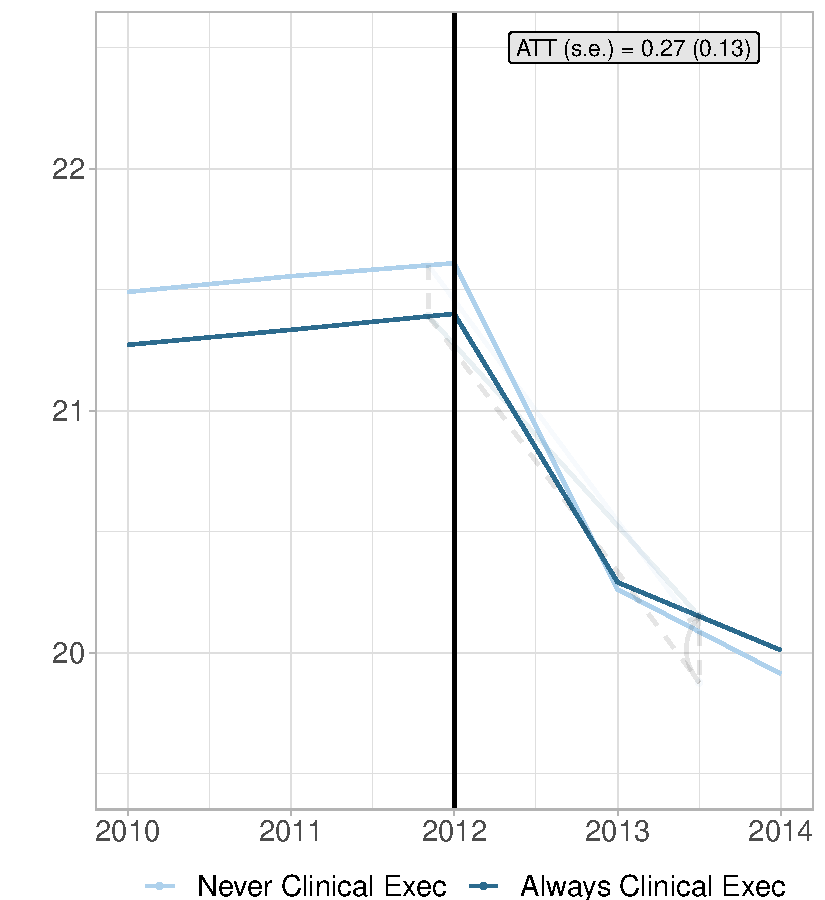
\includegraphics[width=.8\textwidth]{Objects/read_md_nomd_synth_graph.pdf}
    \end{column}
        \begin{column}{0.5\textwidth}
        \centering
        Mortality
        
        \vspace{1mm}
        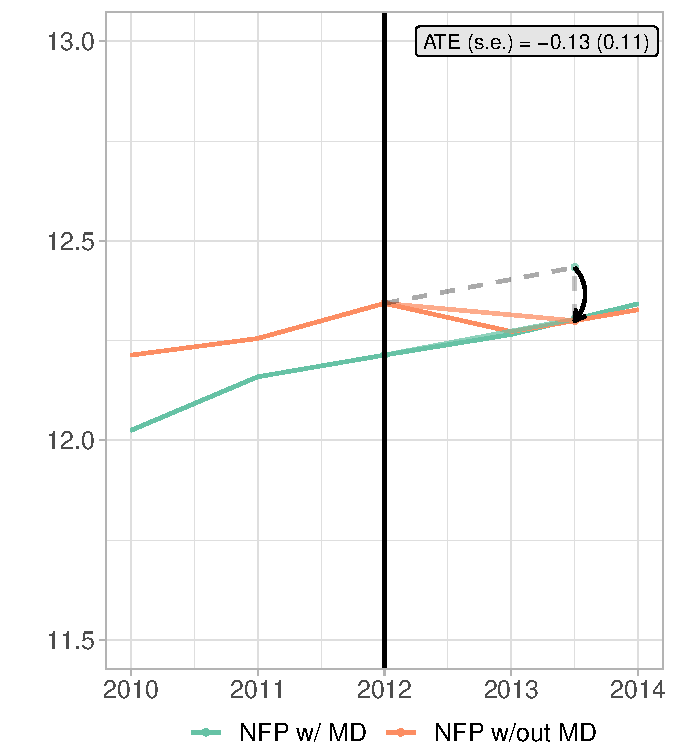
\includegraphics[width=.8\textwidth]{Objects/mort_md_nomd_synth_graph.pdf}
    \end{column}
\end{columns}
\end{frame}

\begin{frame}{Are non-clinical execs more profit driven?}
\begin{block}{}
    Compare each type of NFP w/ for-profit
\end{block}
\begin{equation*}
    y_{ht} = \beta \text{ treat}_{ht} + \gamma_{h} + \delta_t + \epsilon_{ht}
\end{equation*}

\begin{figure}[ht!]
    \begin{center}
 \begin{tabular}{| m{18em} |}
 \hline
 Main Analysis:\\ [0.5ex]
 \hline\hline 
 \vspace{2mm}
 Treat: \hspace{20mm} NFP w/out MD \\
 \vspace{2mm} 
 Comparison: \hspace{8mm} NFP w/ MD  \\
 [1ex]
 \hline
 \end{tabular}
\hfil   %<---
 
\medskip

\vspace{2mm}


  \begin{tabular}{|m{18em}|}
 \hline
 Comparison 1:\\ [0.5ex]
 \hline\hline
 \vspace{2mm}
 Treat: \hspace{20mm} For-Profit \\
 \vspace{2mm}
 Comparison: \hspace{8mm} NFP w/ MD  \\
 [1ex]
 \hline
 \end{tabular}
\hfil   %<---
  \begin{tabular}{|m{18em}|}
 \hline
 Comparison 2:\\ [0.5ex]
 \hline\hline
 \vspace{2mm}
 Treat:  \hspace{20mm} For-Profit \\
 \vspace{2mm}
 Comparison:  \hspace{8mm} NFP w/out MD  \\
 [1ex]
 \hline
 \end{tabular}
 \end{center}
 \end{figure}

    
\end{frame}

\begin{frame}{Compare to FP: Readmissions}
\begin{columns}
    \begin{column}{0.5\textwidth}
        \centering
        FP vs. NFP w/ MD Exec\\\vspace{2mm}
        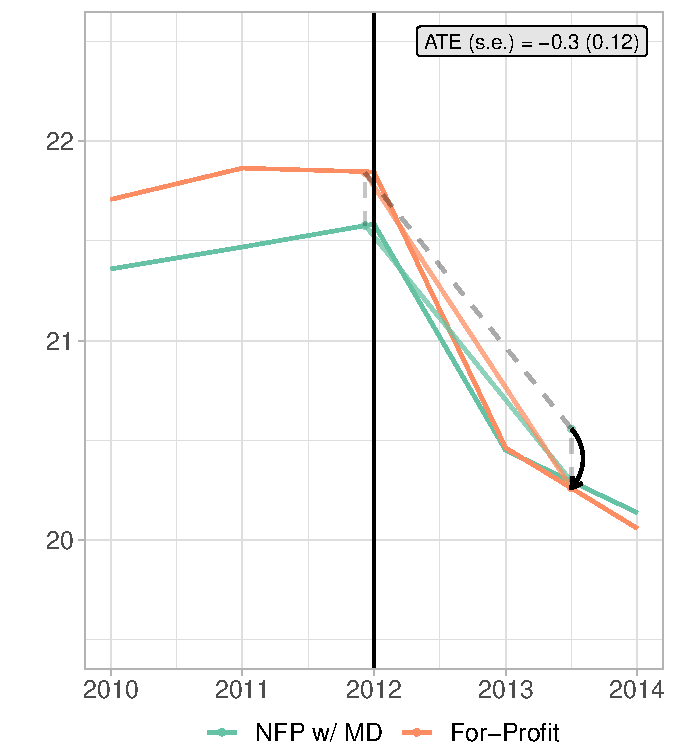
\includegraphics[width=.75\textwidth]{Objects/read_fp_md_synth_graph.pdf}
    \end{column}
        \begin{column}{0.5\textwidth}
        \centering
        FP vs. NFP w/out MD Exec

        \vspace{2mm}
        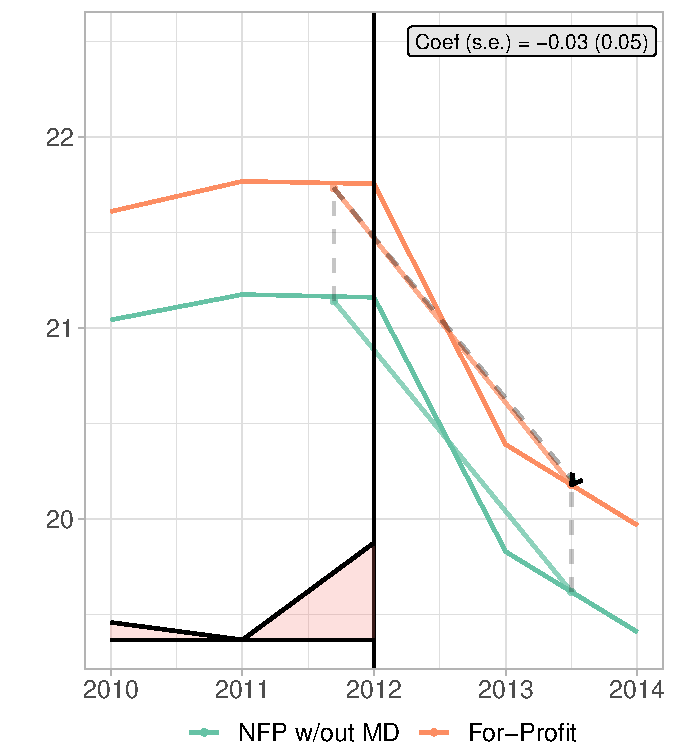
\includegraphics[width=.75\textwidth]{Objects/read_fp_nomd_synth_graph.pdf}
    \end{column}
\end{columns}
\end{frame}


\begin{frame}{Compare to FP: Mortality}
\begin{columns}
    \begin{column}{0.5\textwidth}
        \centering
        FP vs. NFP w/ MD Exec\\\vspace{2mm}
        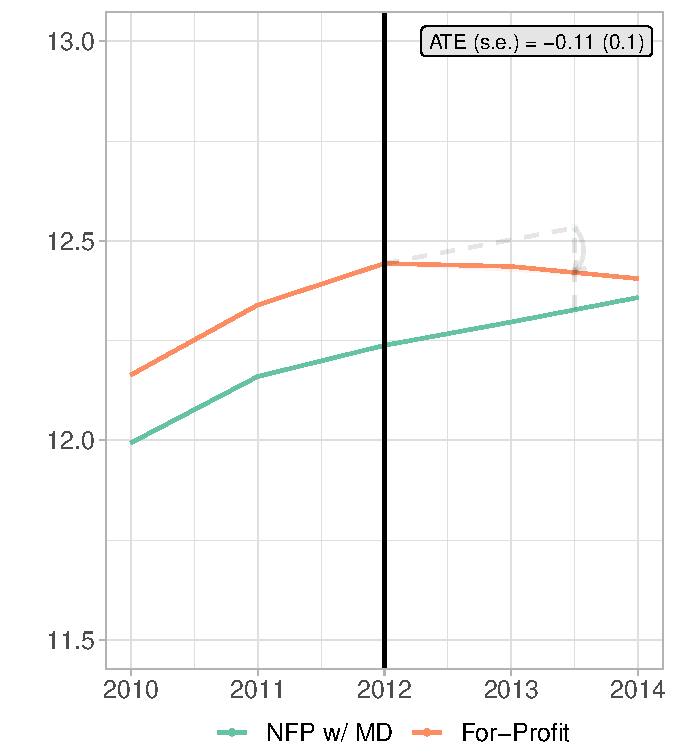
\includegraphics[width=.75\textwidth]{Objects/mort_fp_md_synth_graph.pdf}
    \end{column}
        \begin{column}{0.5\textwidth}
        \centering
        FP vs. NFP w/out MD Exec

        \vspace{2mm}
        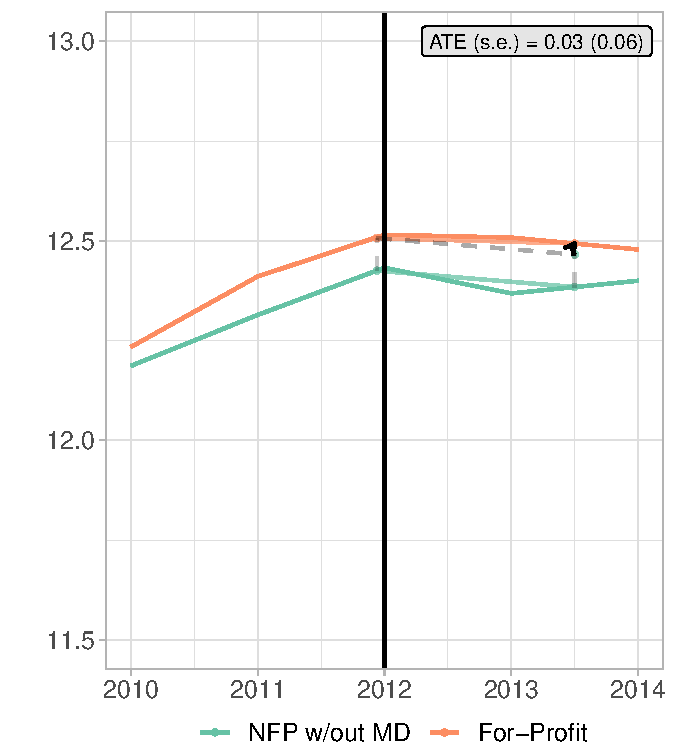
\includegraphics[width=.75\textwidth]{Objects/mort_fp_nomd_synth_graph.pdf}
    \end{column}
\end{columns}
\end{frame}

\begin{frame}{Signalling vs. Managing?}\label{sigman}
    \vspace{7mm}

   Are clinical executives signal of objectives or do they change objectives?
   
   \vspace{7mm}
   
\begin{block}{}
    Include hospitals with change in propensity to hire executive MD
    \begin{itemize}
        \item leverage timing of changes
        \item requires changes not endogenous with P4P incentives \hyperlink{execchanges}{\beamerbutton{change analysis}}
    \end{itemize}
\end{block}
\btVFill\pause

\begin{figure}[ht!]
    \begin{center}
 \begin{tabular}{| m{18em} |}
 \hline
 Signalling:\\ [0.5ex]
 \hline\hline 
 \vspace{2mm}
 Treat: \hspace{20mm} Never MD Exec \\
 \vspace{2mm} 
 Comparison: \hspace{8mm} Ever MD Exec  \\
 [1ex]
 \hline
 \end{tabular}
\hfil   %<---
 \begin{tabular}{|m{18em}|}
 \hline
 Managing:\\ [0.5ex]
 \hline\hline
 \vspace{2mm}
 Treat: \hspace{20mm} MD Exec (not 2012) \\
 \vspace{2mm}
 Comparison: \hspace{8mm} MD Exec 2012  \\
 [1ex]
 \hline
 \end{tabular}

 \end{center}
 \end{figure}
\end{frame}

\begin{frame}{Signalling vs. Managing?}

\footnotesize
\begin{table}[ht!]
\centering
\begin{tabular}[t]{lcccc}
\toprule
\multicolumn{1}{c}{ } & \multicolumn{2}{c}{\underline{Weighted Avg. Readmission Rate}} & \multicolumn{2}{c}{\underline{Weighted Avg. Mortality Rate}} \\
\addlinespace
 & (1) & (2) & (3) & (4)\\
\midrule
Never MD Exec x Post Programs & 0 &  & -0.06 & \\
 & (0.06) &  & (0.06) & \\
Ever MD (not in 2012) &  & -0.19$^{*}$ &  & -0.1\\
 \hspace{3mm} x Post Programs &  & (0.09) &  & (0.08)\\
 &  &  &  & \\
\addlinespace
\textbf{Comparison Group:} &  &  &  & \\
Ever MD Exec & $\checkmark$ &  & $\checkmark$ & \\
Has MD Exec 2012 &  & $\checkmark$ &  & $\checkmark$\\
 &  &  &  & \\
Observations & 3,925 & 1,845 & 3,910 & 1,840\\
\bottomrule
\end{tabular}
\end{table}


\end{frame}

\begin{frame}{Conclusion}
I examine whether having clinical experience on a leadership team affects how the hospital responds to a change in incentives

\vspace{5mm}

\begin{enumerate}
    \item Hospitals w/out clinical executives respond more aggressively to P4P incentives \pause

    \vspace{3mm}
    
    \item Hospitals w/out clinical executive act more like for-profits \pause

    \vspace{3mm}

    
    \item Seems to be driven by differences in management, not a signal of underlying objectives
\end{enumerate}
\end{frame}

\begin{frame}{}
    \Large
    \centering

    \textcolor{sage}{Thank you!}

    \vspace{5mm}

    \textcolor{sage}{hanna.glenn@emory.edu}

\end{frame}



\begin{frame}[noframenumbering]{Tax Form 990s: Collection}\label{990s}

\vspace{5mm}
    \begin{wideitemize}
        \item Forms stored at ProPublica
        \item Use API to collect EIN numbers from NFPs classified as hospitals 
        \item For each EIN, download pdf locally using URLs and API
        \item Manually collect those that get skipped
    \end{wideitemize}
    \btVFill

    \hyperlink{clinexecs}{\beamerbutton{back}}
\end{frame}

\begin{frame}[noframenumbering]{Tax Form 990s: Matching}
\vspace{5mm}
    Need to match to AHA data to get other hospital characteristics
    \vspace{3mm}
    \begin{wideitemize}
        \item Crosswalks from EIN to AHA ID or Medicare number do not exist
        \item Best I can do is match based on name of hospital and location
        \item I match based on exact name matches in the same state (800 matches)
        \item Then I match based on rough name matches in the same state (300 matches)
        \item Manually match as many as I can (100 matches)
    \end{wideitemize}
    \btVFill

    \hyperlink{clinexecs}{\beamerbutton{back}}
\end{frame}

\begin{frame}[noframenumbering]{Tax Form 990s: Text Extraction and Cleaning}
\vspace{5mm}
    \begin{wideitemize}
        \item Extract text from all pages with executives and key directors
        \item find name locations based on common appearances of Census first and last names
        \item Locate position and title that appear closest to the name
    \end{wideitemize}

    \btVFill

    \hyperlink{clinexecs}{\beamerbutton{back}}
\end{frame}

\begin{frame}[noframenumbering]{Executive Team Statistics}\label{execstats}

\vspace{10mm}
    \begin{table}[ht!]
    \centering
    \begin{tabular}[t]{lcccc}
    \toprule
    Variable & Mean & Std. Dev. & Min & Max\\
    \midrule
    Number Executives & 3.91 & 2.75 & 1 & 27\\
    Number MD Executives & 0.40 & 0.73 & 0 & 6\\
    \hspace{5mm}Percent MD Execs & 0.09 & 0.17 & 0 & 1\\
    No Change in MD Hiring Propensity & 0.61 & 0.49 & 0 & 1\\
    \bottomrule
    \end{tabular}
    \end{table}

    \btVFill

    \hyperlink{clinexecs}{\beamerbutton{back}}
\end{frame}

\begin{frame}[noframenumbering]{Endogenous Executive Changes?}\label{execchanges}
\small
    \begin{table}[ht!]
   \centering
   \begin{tabular}{lcccccc}
      \toprule
       & \multicolumn{3}{c}{Change in Any MD} & \multicolumn{3}{c}{Change in Num. MDs}\\
                                      & (1)    & (2)    & (3)           & (4)    & (5)    & (6)\\  
      \midrule 
      Ever Penalized HRRP x Post 2011 & 0.01   &        &               & 0.02   &        &   \\   
                                      & (0.02) &        &               & (0.02) &        &   \\   
      Ever Payment HVBP x Post 2011   &        & 0.00   &               &        & 0.02   &   \\   
                                      &        & (0.02) &               &        & (0.02) &   \\   
      2011                            &        &        & -0.02         &        &        & -0.02\\   
                                      &        &        & (0.02)        &        &        & (0.02)\\   
      2012                            &        &        & -0.05$^{**}$  &        &        & -0.04$^{*}$\\   
                                      &        &        & (0.02)        &        &        & (0.02)\\   
      2013                            &        &        & -0.04$^{**}$  &        &        & -0.03\\   
                                      &        &        & (0.02)        &        &        & (0.02)\\   
      2014                            &        &        & -0.05$^{***}$ &        &        & -0.03\\   
                                      &        &        & (0.02)        &        &        & (0.02)\\   
       \\
      Observations                    & 3,808  & 3,808  & 3,808         & 3,808  & 3,808  & 3,808\\  
      \bottomrule
   \end{tabular}
\end{table}

\hyperlink{sigman}{\beamerbutton{back}}

\end{frame}

\begin{frame}[noframenumbering]{2012 Pay-for-Performance Policies}\label{policies}
    \vspace{3mm}

    Hospital Readmissions Reduction Program:
    \begin{itemize}
        \item Penalty for high readmissions for given conditions: heart attack, heart failure, pneumonia
        \item If penalized, pay 1-3\% reimbursement for \textit{every} Medicare patient
        \begin{itemize}
            \item 19\% of the US population is on Medicare
            \item 21\% of health care is paid by Medicare
        \end{itemize}
        
    \end{itemize}

    \vspace{5mm}

    Hospital Value Based Purchasing Program:
    \begin{itemize}
        \item Rewarded based on quality compared to other hospitals and whether quality improves over time
        \item All hospitals pay in, hospitals above average receive the payment
    \end{itemize}
    \btVFill

    \begin{block}{}
        Exogenous shocks to hospitals: predetermined leadership teams are not correlated with the incentive change \hyperlink{policies}{\beamerbutton{back}}
    \end{block}
\end{frame}

\begin{frame}[noframenumbering]{Summary Stats: Hospital Characteristics}
    \begin{table}[ht!]
\centering
\begin{tabular}[t]{lcccc}
\toprule
Variable & Mean & Std. Dev. & Min & Max\\
\midrule
\addlinespace[0.3em]
\multicolumn{5}{l}{\textbf{Hospital Characteristics}}\\
\hspace{1em}Number Beds & 162.15 & 211.79 & 10 & 9,900\\
\hspace{1em}Num. Patients AMI & 143.23 & 198.32 & 1 & 1,667\\
\hspace{1em}Num. Patients HF & 325.50 & 337.01 & 1 & 2,547\\
\hspace{1em}Num. Patients Pneumonia & 283.11 & 230.93 & 1 & 2,032\\
\hspace{1em}Academic Med. Center & 0.25 & 0.43 & 0 & 1\\
\hspace{1em}Physician Owned & 0.08 & 0.27 & 0 & 1\\
\hspace{1em}System Affiliated & 0.57 & 0.50 & 0 & 1\\
\hspace{1em}Case Mix Index & 1.44 & 0.26 & 0.58 & 3.75\\
\bottomrule
\end{tabular}
\end{table}
\end{frame}

\begin{frame}[noframenumbering]{Summary Stats: Penalty/Payment}
    \begin{table}[ht!]
\centering
\begin{tabular}[t]{lcccc}
\toprule
Variable & Mean & Std. Dev. & Min & Max\\
\midrule
\addlinespace[0.3em]
\multicolumn{5}{l}{\textbf{Penalty/Payment Variables}}\\
\hspace{1em}Ever Received HVBP Incentive & 0.77 & 0.42 & 0.00 & 1.00\\
\hspace{1em}Penalized for AMI & 0.04 & 0.19 & 0.00 & 1.00\\
\hspace{1em}Penalized for HF & 0.05 & 0.22 & 0.00 & 1.00\\
\hspace{1em}Penalized for Pneumonia & 0.06 & 0.24 & 0.00 & 1.00\\
\hspace{1em}Penalized for AMI + HF & 0.05 & 0.23 & 0.00 & 1.00\\
\hspace{1em}Penalized for AMI + Pneumonia & 0.15 & 0.36 & 0.00 & 1.00\\
\hspace{1em}Penalized for HF + Pneumonia & 0.15 & 0.36 & 0.00 & 1.00\\
\hspace{1em}Penalized for All Conditions & 0.30 & 0.46 & 0.00 & 1.00\\
\bottomrule
\end{tabular}
\end{table}
\end{frame}

\begin{frame}[noframenumbering]{Summary Stats: Outcomes}
    \begin{table}[ht!]
\centering
\begin{tabular}[t]{lcccc}
\toprule
Variable & Mean & Std. Dev. & Min & Max\\
\midrule
\addlinespace[0.3em]
\multicolumn{5}{l}{\textbf{Readmission Outcome Variables}}\\
\hspace{1em}Weighted Avg. Readmission Rate & 20.76 & 1.86 & 15.10 & 29.09\\
\hspace{1em}AMI Readmission Rate & 19.14 & 1.53 & 14.50 & 26.30\\
\hspace{1em}HF Readmission Rate & 24.15 & 2.08 & 16.60 & 33.60\\
\hspace{1em}Pneum. Readmission Rate & 18.15 & 1.61 & 13.60 & 24.80\\
\addlinespace[0.3em]
\multicolumn{5}{l}{\textbf{Mortality Outcome Variables}}\\
\hspace{1em}Weighted Avg. Mortality Rate & 12.37 & 1.42 & 7.23 & 20.25\\
\hspace{1em}AMI Mortality Rate & 15.60 & 1.60 & 10.10 & 22.70\\
\hspace{1em}HF Mortality Rate & 11.66 & 1.58 & 6.00 & 18.00\\
\hspace{1em}Pneum. Mortality Rate & 12.01 & 1.88 & 6.40 & 22.10\\
\\
Num. Hospitals & 1560.00 &  &  & \\
\bottomrule
\end{tabular}
\end{table}
\end{frame}

\begin{frame}[noframenumbering]{Sub-sample Summary Stats: Hospital Characteristics}
    \begin{table}[ht!]
    \small
\centering
\begin{tabular}[t]{lcccccl}
\toprule
 & (1) & (2) & (3) & (4) & (5) & (6)\\
\addlinespace[0.3em]
\multicolumn{2}{c}{ } & \multicolumn{3}{c}{Not-for-Profit} & \multicolumn{2}{c}{Stable Not-for-Profit} \\
\cmidrule(l{3pt}r{3pt}){3-5} \cmidrule(l{3pt}r{3pt}){6-7}
Variable & For-Profit & All & Ever MD & Never MD & Ever MD & Never MD\\
\midrule
\addlinespace[0.3em]
\multicolumn{7}{l}{\textbf{Hospital Characteristics}}\\
\hspace{1em}Number Beds & 155 & 149 & 232 & 115 & 216 & 115\\
\hspace{1em}Num. Patients AMI & 112 & 138 & 228 & 109 & 209 & 109\\
\hspace{1em}Num. Patients HF & 276 & 299 & 475 & 266 & 453 & 265\\
\hspace{1em}Num. Patients Pneum. & 234 & 258 & 394 & 256 & 390 & 256\\
\hspace{1em}Academic Med. Center & 0.17 & 0.27 & 0.40 & 0.24 & 0.48 & 0.24\\
\hspace{1em}Physician Owned & 0.19 & 0.01 & 0.01 & 0.01 & 0.03 & 0.01\\
\hspace{1em}System Affiliated & 0.90 & 0.60 & 0.60 & 0.43 & 0.44 & 0.28\\
\hspace{1em}Case Mix Index & 1.44 & 1.44 & 1.50 & 1.37 & 1.52 & 1.37\\
\addlinespace[0.3em]
Num. Hospitals & 708 & 852 & 384 & 468 & 56 & 465\\
\bottomrule
\end{tabular}
\end{table}
\end{frame}

\begin{frame}[noframenumbering]{Sub-sample Summary Stats: Penalty/Payment}
    \begin{table}[ht!]
    \footnotesize
\centering
\begin{tabular}[t]{lcccccl}
\toprule
 & (1) & (2) & (3) & (4) & (5) & (6)\\
\addlinespace[0.3em]
\multicolumn{2}{c}{ } & \multicolumn{3}{c}{Not-for-Profit} & \multicolumn{2}{c}{Stable Not-for-Profit} \\
\cmidrule(l{3pt}r{3pt}){3-5} \cmidrule(l{3pt}r{3pt}){6-7}
Variable & For-Profit & All & Ever MD & Never MD & Ever MD & Never MD\\
\midrule
\addlinespace[0.3em]
\multicolumn{7}{l}{\textbf{Penalty/Payment Variables}}\\
\hspace{1em}Ever Received HVBP & 0.87 & 0.62 & 0.81 & 0.59 & 0.71 & 0.59\\
\hspace{1em}Penalized for AMI & 0.03 & 0.03 & 0.05 & 0.03 & 0.04 & 0.03\\
\hspace{1em}Penalized for HF & 0.06 & 0.06 & 0.04 & 0.05 & 0.05 & 0.05\\
\hspace{1em}Penalized for Pneumonia & 0.06 & 0.05 & 0.09 & 0.04 & 0.09 & 0.05\\
\hspace{1em}Penalized for AMI + HF & 0.06 & 0.04 & 0.06 & 0.04 & 0.05 & 0.04\\
\hspace{1em}Penalized for AMI + Pneum. & 0.04 & 0.05 & 0.07 & 0.05 & 0.07 & 0.05\\
\hspace{1em}Penalized for HF + Pneum. & 0.20 & 0.13 & 0.12 & 0.12 & 0.11 & 0.12\\
\hspace{1em}Penalized for All Conditions & 0.36 & 0.22 & 0.31 & 0.21 & 0.30 & 0.21\\
\addlinespace[0.3em]
Num. Hospitals & 708 & 852 & 384 & 468 & 56 & 465\\
\bottomrule
\end{tabular}
\end{table}
\end{frame}

\begin{frame}[noframenumbering]{Sub-sample Summary Stats: Outcomes}
    \begin{table}[ht!]
    \footnotesize
\centering
\begin{tabular}[t]{lcccccl}
\toprule
 & (1) & (2) & (3) & (4) & (5) & (6)\\
\addlinespace[0.3em]
\multicolumn{2}{c}{ } & \multicolumn{3}{c}{Not-for-Profit} & \multicolumn{2}{c}{Stable Not-for-Profit} \\
\cmidrule(l{3pt}r{3pt}){3-5} \cmidrule(l{3pt}r{3pt}){6-7}
Variable & For-Profit & All & Ever MD & Never MD & Ever MD & Never MD\\
\midrule
\addlinespace[0.3em]
\multicolumn{7}{l}{\textbf{Readmission Outcome Variables}}\\
\hspace{1em}Weighted Avg. Readmission & 21.09 & 20.47 & 20.63 & 20.44 & 20.79 & 20.44\\
\hspace{1em}AMI Readmission Rate & 19.19 & 19.13 & 19.01 & 19.23 & 18.90 & 19.23\\
\hspace{1em}HF Readmission Rate & 24.42 & 23.99 & 23.81 & 24.08 & 23.93 & 24.08\\
\hspace{1em}Pneum. Readmission Rate & 18.30 & 18 & 18.10 & 18 & 18.26 & 18\\
\addlinespace[0.3em]
\multicolumn{7}{l}{\textbf{Mortality Outcome Variables}}\\
\hspace{1em}Weighted Avg. Mortality Rate & 12.38 & 12.29 & 12.36 & 12.36 & 12.34 & 12.36\\
\hspace{1em}AMI Mortality Rate & 15.82 & 15.46 & 15.29 & 15.61 & 15.17 & 15.61\\
\hspace{1em}HF Mortality Rate & 11.52 & 11.67 & 11.71 & 11.83 & 11.57 & 11.82\\
\hspace{1em}Pneum. Mortality Rate & 12.08 & 11.98 & 11.83 & 12.07 & 12 & 12.06\\
\addlinespace[0.3em]
Num. Hospitals & 708 & 852 & 384 & 468 & 56 & 465\\
\bottomrule
\end{tabular}
\end{table}
\end{frame}



\end{document}